

\section{Introduction}
\label{sec:introduction}

\vspace{-1em} %This is a trick to avoid PDF links issues.

The quantitative understanding of the physical world is an essential goal of geoscience research. We use mathematical abstractions to represent the behavior of systems under static and dynamic conditions; and we define properties such as density and elastic moduli to characterize the capacity of materials to absorb or transmit forces in static and dynamic processes. In seismology and geophysics, our understanding of physical phenomena associated with earthquakes, their genesis, and effects, depends, in good measure, on our knowledge and accurate representation of the geometry and material properties of the Earth's structure, as well as on our capacity to represent the mechanical characteristics of the earthquake rupture process and the subsequent propagation of seismic waves through the earth. Computational geoscientists use stress conditions and dynamic rupture models to describe faulting processes, and seismic velocity and attenuation models, along with wave propagation principles, to calculate characteristics of earthquake ground motions. Initial stress models and seismic velocity models are therefore the basic input used in earthquake ground motion simulation.

We are interested in how seismic velocity models are built and made available to geoscientists, and how these models can help advance physics-based earthquake science. We utilize modeling approaches based on deterministic numerical techniques---such as the finite element, finite difference, or spectral element methods---to simulate the ground motion in ways that incorporate the physics of earthquake processes explicitly. That is, methods that explicitly solve the associated wave propagation problem. The use of physics-based earthquake simulation has increased considerably over the last two decades thanks to the growth in capacity and availability of high-performance computing (HPC) facilities and applications \citep[e.g.,][]{Aagaard_2008_BSSA2, Olsen_2009_GRL, Bielak_2010_GJI, Cui_2010_Proc}. These simulations have important applications in seismology and earthquake engineering for purposes such as the assessment of regional seismic hazard \citep[e.g.,][]{Graves_2011_PAG}.

Recent earthquake simulations have shown the importance of velocity models in the accuracy of simulation results \citep[e.g.,][]{Taborda_2014_BSSA}. Numerous seismic velocity models have been built for specific regional or local structures and used in particular simulations over the years \citep[e.g.,][]{Frankel_1992_BSSA, Brocher_2008_BSSA, Graves_2008_BSSA}. The concept of community velocity models (CVMs) has emerged from broad use of velocity models in earthquake simulations. CVMs are seismic velocity models that have been developed, maintained, improved, and used by a community of interested investigators. Some examples of CVMs for the regions of southern and northern California, Utah, and the central United States are those models developed by \citet{Kohler_2003_BSSA}, \citet{Suss_2003_JGR}, \citet{Brocher_2006_Proc}, \citet{Magistrale_2006_Tech}, \citet{Plesch_2011_SCEC}, and \citet{RamirezGuzman_2012_BSSA}. 

CVMs are typically distributed in the form of datasets or collections of files, or in the form of computer programs that can dynamically operate on these datasets and files to provide information about the geometry and material properties of the crust in a particular region. However, these datasets and computer programs have not been designed consistently from a computational perspective. For example, not all CVM's define the same material properties, or use the same geographical projection. In addition, recent advances in earthquake simulations, powered by the increasing capability of supercomputers, have increased significantly the computational demand placed on CVMs as input to these simulations.

This paper presents the Unified Community Velocity Model (UCVM), a software framework developed and maintained by the Southern California Earthquake Center (SCEC), designed to provide standardized and computationally efficient access to seismic velocity models. UCVM is a collection of software tools and application programming interfaces (APIs) that facilitate access to the material properties stored in CVMs. Although UCVM was conceived as a tool to aid physics-based earthquake ground-motion simulation and regional seismic hazard assessment, it can be, and has been used in other geoscience and engineering applications. Here, we describe the development of UCVM and its various software components and features, including its use in high-performance parallel computers, and present examples of recent applications of UCVM tools in geoscience and earthquake engineering research.



\section{Community Velocity Models}
\label{sec:cvms}

\textit{
\color{blue}
This section will present how CVMs work and the various CVMs available to the community today. It will basically explain that CVMs provide the triplets of Vs, Vp and density, and, as an example, we can expand on a description of CVM-S and CVM-H, including their variations CVM-SI and CVM-H+GTL.
}

\section{The UCVM Software Framework}\label{sec:ucvm}

\subsection{Overview}
The most significant functionality provided by UCVM is the ability to query a wide array of community velocity models for material properties in a standard way. Once a velocity model has been successfully integrated with UCVM, the framework can be utilized to query for the primary and shear seismic wave velocities ($Vp$, $Vs$) as well as the soil/rock density ($\rho$) at any geographic point within that model. The original model's local coordinate system and map projection are concealed behind a generic interface that instead allows queries by geographic latitude and longitude along with a vertical z-coordinate. The z-axis may be defined as either depth below the free surface or elevation relative to mean sea level.

To support this flexible query mechanism consistently across all models, UCVM includes a high-resolution digital elevation model (DEM). The DEM is synthesized from the USGS National Elevation Dataset (TODO: cite USGS NED) and the ETOPO1 Global Relief Model (TODO: cite ETOPO1). It currently spans the State of California along with portions of surrounding States. 
\begin{figure}
\centering
\epsfig{file=UCVM_Tiling_Concept.pdf,scale=0.35}
\caption{Tiling of velocity models (TODO: Redo/cleanup this figure).}\label{fig:tiling}
\end{figure}

The framework further extends the standardized interface by allowing multiple velocity models to be aggregated into a single composite model. Composition is accomplished by tiling two or more velocity models in three dimensions according to a user-specified priority ordering. Under this scheme, a query point is submitted sequentially to each velocity model within the ordered list that comprises the composite. The first model to return valid velocity data for the point is considered to have fulfilled the data request and subsequent models are not queried. Thus, overlap among the individual models is acceptable and their relative priority ordering arbitrates which one satisfies any given query. Generally, no smoothing is performed at the interfaces between models (an exception is interpolation between a geotechnical layer and a crustal model as discussed later in this paper). This tiling concept is illustrated in Figure \ref{fig:tiling}.

Community velocity models vary widely in their area of coverage, depth extent, and resolution. UCVM is flexible in its support for such variability. However, in order to better accommodate high frequency ground motion simulations, it categorizes models into two general groups: crustal models, and geotechnical layers (GTLs). Crustal models provide subsurface seismic wave velocities associated with basin, crust, and mantle structures. These models may potentially extend to many tens of kilometers below the Earth's surface yet do so at coarse resolutions (TODO: cite CVM-H, CVM-S). Geotechical layers, in contrast, provide velocities for only the near-surface (typically a few hundred meters) at very high resolution (TODO: cite Ely Vs30 GTL). Ground motion simulations, in particular, rely on high-resolution near-surface velocities and therefore a GTL serves to supplement the coarser data provided by crustal models.
\begin{figure}
\centering
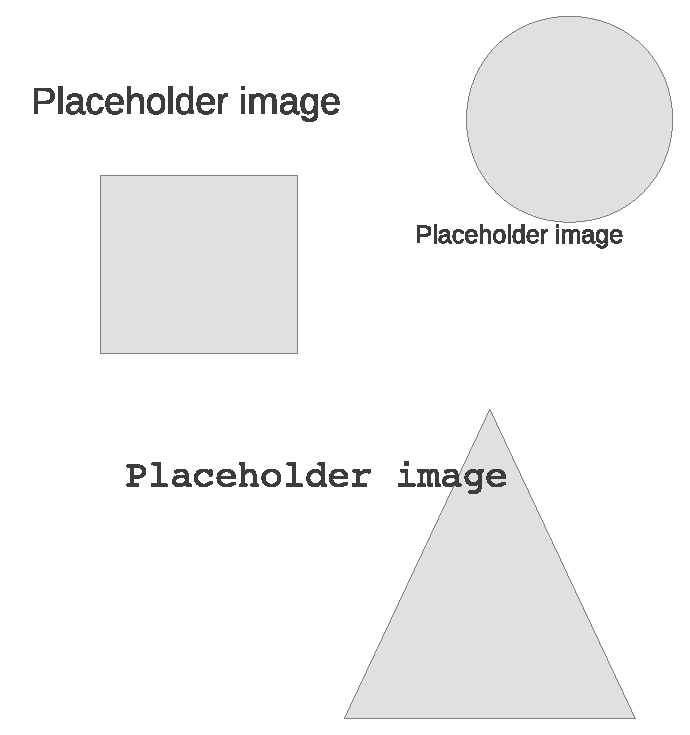
\epsfig{file=place_holder.pdf,scale=0.35}
\caption{Interpolation of GTL and crustal model.}\label{fig:interpolation}
\end{figure}

When querying a set of velocity models that includes at least one GTL, the tiling mechanism described previously is enhanced to perform limited interpolation. The framework independently composes the GTLs and the crustal models into a composite GTL and composite crustal model, respectively, using the tiling technique. An interpolation zone is then defined along the z-axis between the two composites. Query points that fall within the zone are assigned an interpolated velocity based on the composite GTL velocity at the top of the zone boundary and the composite crustal model velocity at the bottom. Both the zone dimensions and interpolation function is selectable by the user. Figure \ref{fig:interpolation} illustrates how this interpolation is performed. The primary motivation for performing interpolation in this particular case is to eliminate near-surface discontinuities between the GTLs and the crustal models which would adversely affect ground motion simulations.
\begin{table}
\centering
\caption{Supported Community Velociy Models}\label{table:supported_models}
\begin{tabular}{|c|c|c|} \hline
Model & Versions & Reference \\ \hline
CVM-H & TBD & TBD \\ \hline
CVM-S & TBD & TBD \\ \hline
TBD & TBD & TBD \\
\hline\end{tabular}
\end{table}

Table \ref{table:supported_models} summarizes the list of community velocity models that have been integrated into UCVM. A single geotechnical layer is currently supported, based on Ely's Vs30-derived algorithm (TODO: cite Ely Vs30-derived GTL). This algorithm procedurally estimates $Vp$, $Vs$, and $\rho$ from the Vs30 velocity at the point of interest. To that end, two separate Vs30 maps are provided for use with the Ely GTL, and each covers the same geographic region as the DEM (namely, California). One map is based on the the Wills and Wald dataset (TODO: cite Wills and Wald), and the other is based on the Yong dataset (TODO: cite Yong). 

\subsection{Command-line Utilities}

The UCVM software framework provides UNIX command-line utilities to interactively query velocity models and construct regular three-dimensional meshes of material properties. These programs are described in the following sections.

\subsubsection{Querying}

The primary command-line tool for extracting material properties is \emph{ucvm\_query}. The typical use case is to invoke the program while specifying the path to the UCVM configuration file and a prioritized list of models to query. Both the configuration file and the pool of available velocity models are setup during the framework installation process. The configuration file allows UCVM to find the necessary resources during runtime, while the model list is a subset of installed models to be used in the current query session.

Once executed, the program loads the necessary models, tiles them in the same order as they were specified on the command-line, and awaits query coordinates from the user. The default format for coordinates is longitude (decimal), latitude (decimal), and depth (meters). Alternatively, elevation may be used for the z coordinate with a command-line option. For each submitted query point, UCVM returns a text line composed of seventeen fields. The first three fields of the output echo the original query coordinates. The next two fields list the surface elevation from the DEM and the Vs30 value from the active Vs30 map. Bilinear interpolation is used to calculate smoothed values at the point of interest since both of these maps are gridded at 250m resolution.

The remaining twelve fields represent three sets of material properties. Each group of material properties is comprised of four fields: the source model whence the material properties were drawn, Vp, Vs, and $\rho$. As UCVM is able to perform limited interpolation between models, both the inputs to the interpolation and the smoothed result are shown for each query point. Thus, the first two parameter groups correspond to the crustal model and GTL that satisfied the query, respectively, while the third parameter group displays the interpolated results. If no GTL is defined, or the query point falls outside of the interpolation zone, the third parameter group simply repeats the results of whichever model satisfied the request. In any case, the framework's final verdict is given in this last parameter group.

As extraction of iso-surfaces based on shear wave velocity is a common and time-consuming application of community velocity models, UCVM offers a specialized query program for this purpose. The iso-surface utility \emph{basin\_query} is invoked in a similar manner to \emph{ucvm\_query}, yet it also allows the user to specify a Vs threshold for the iso-surface and a step size for successive query points along the z-axis. Query points are specified in longitude and latitude coordinates, and the program iteratively queries the tiled velocity models from the surface to a maximum depth using the provided step-size. Four fields are returned for each query point; the first two echo the original geographic coordinates while the remaining two fields report the minimum and maximum depths where the Vs threshold is crossed.

\subsubsection{Meshing}
Modern seismic wave propagation simulations often require a three-dimensional input mesh which describes the wave velocities and soil density for the entire simulation region. Constructing a mesh can be a time-consuming and error-prone prerequisite to executing a simulation. The UCVM framework assists in this respect by providing command-line utilities for generating three-dimensional meshes, in either structured binary or netCDF format, and Etree databases (TODO: cite Etree library). The binary meshes and the Etree databases may be used with the simulation codes AWP-ODC (TODO: cite APW-ODC) and Hercules (TODO: cite Hercules), respectively.

The AWP-ODC wave propagation software utilizes a mesh format consisting of a regular grid of cells at uniform resolution. Nominally, each cell contains the material properties Vp, Vs, and $\rho$, which are extracted directly from one or more community velocity models. The framework utility \emph{ucvm2mesh} performs this extraction and produces an output mesh of the correct format. The program accepts a configuration file at runtime which describes the extent of the Earth's surface and crust to be gridded, the grid spacing, and the list of velocity models to be used for extraction. The mesh grid is defined by first applying a two-dimensional map projection whose origin is a geographic coordinate, and whose axes are the projection axes (which may be optionally rotated). As UCVM employs the Proj4 software library (TODO: cite Proj4), virtually every standard map projection is supported. The number of elements along each axis and the grid spacing in projection units fully define the maximum extents of the mesh. This two-dimensional grid is then replicated along the Z-axis at intervals of the grid spacing to yield the full mesh grid. The UCVM framework converts each point in this grid from map coordinates back to geographic coordinates, queries them by tiling all velocity models in the same manner as \emph{ucvm\_query}, and builds the mesh.

The Hercules wave propagation software eliminates the need for an input mesh and instead utilizes an Etree database. The Etree database format is an octree of material properties that minimally spans the simulation region, yet is typically much larger. Since it is based on the octree data structure, the database supports variable resolution octants and an efficient storage format. The Etree library augments these advantages by also providing an efficent querying mechanism for extracting information. An Etree database is intended to be re-usable in different simulations, and each is rated for a maximum supported simulation frequency. 

The UCM framework utility \emph{ucvm2etree} is employed to generate an Etree database for use with Hercules. The program accepts a configuration file that defines the extent of the Earth's surface and crust to span, the desired maximum simulation frequency to support, and the list of velocity models to be used for extraction. Due to the differences between this database format and that of a regular mesh, the extents are specified in an alternative format to that used in the \emph{ucvm2mesh} utility. A two-dimensional map projection is applied as before, but no grid is explicitly defined; instead, the desired total length along each dimension in projection units is used to derive a large bounding box for the Etree in projection coordinates. This three-dimensional bounding box is then divided into a two-dimensional logical array of rectangular cuboids (columns) of fixed size. This decomposition into columns assists in parallelization since the material properties for a particular column can be extracted independently from the others.

For each column of the bounding box, \emph{ucvm2etree} queries the material properties Vp, Vs, and $\rho$ from the tiled set of velocity models. The material properties are inserted into the database in a top-down fashion, starting from the surface and ending at the maximum depth. As the program moves down the Z-axis, the octant size is adaptively calculated by the following formula.
\begin{equation*}
s_{octant} = \frac{l_{max}}{ 2^{\left( \left\lceil \log_{2}(\frac{l_{max}}{s_{max}}) \right\rceil \right)} }
\end{equation*}
The variable $l_{max}$ is the length of the longest side of the Etree bounding box, and $s_{max}$ is the maximum possible octant size that can support the local minimum shear wave velocity. This latter value is determined by the following formula.
\begin{equation*}
s_{max} = \frac{v_{min}}{m f_{max}}
\end{equation*}
The variable $v_{min}$ is the minimum shear wave velocity encountered in a sampled two-dimensional slice of the column at this depth. The values $f_{max}$ and $m$ represents the maximum frequency and points per wavelength, respectively, that were specified by the user. This calculation yields a valid octant size for the Etree and ensures that each column is extracted at a resolution which supports the maximum simulation frequency.

Mesh extraction to the netCDF format is supported with the post-processing utility \emph{mesh2netcdf}. This utility takes as input a structured binary mesh that was previously extracted with \emph{ucvm2mesh} and converts it into the netCDF format.

Modern seisic simulations require input meshes of very large size, often consisting of billions of elements. Extraction of these large meshes is a formidible task when performed in a serial manner. Parallel versions of \emph{ucvm2mesh} and \emph{ucvm2etree} are provided by the UCVM framework to accelerate the mesh generation process. These programs utilize the Message Passing Inteface (MPI) to divide the mesh or Etree region into a collection of smaller chunks, extract each chunk independently on a different computer processor, and combine the intermediate results into the final mesh or Etree.

The program \emph{ucvm2mesh-mpi} is the parallel implementation for generating structured binary meshes. It assumes the presence of a correctly configured MPI environment and accepts a configuration file when executed. This configuration file differs slightly from the serial version in that it contains additional entries to instruct how the grid points of the mesh are disaggregated and distributed among the available compute nodes for extraction.

Extraction of an Etree database in a parallel fashion is a more difficult task as the Etree library does not provide a parallel mechanism for inserting octants into the database. Although extraction can be readily parallelized, insertion of the material properties into the final Etree must be done serially. The most efficient insertion method supported by the library is the octant append operation, however, this requires that each octant be inserted in location code order. Since the Etree extraction process is adaptive based on local shear wave velocity, it is impossible to determine apriori the full list of sorted octant locations. Instead, all the octants must be extracted, sorted by location code, then inserted sequentially into the Etree database. The framework provides a set of three MPI applications to accomplish this multi-step build process: \emph{ucvm2etree-extract-MPI}, \emph{ucvm2etree-sort-MPI}, and \emph{ucvm2etree-merge-MPI}.


\subsection{Application Programming Interface}

TODO: how to interface programmatically with UCVM

\subsubsection{Architecture}

TODO: describe architecture: proj4, etree library, layering/dependencies of framework

\subsubsection{Extensibility}

TODO: describe how to support new DEMs, Vs30 maps, and models

The DEM may be modified to cover any arbitrary region of the Earth's surface, provided adequate resolution elevation datasets exist.

Alternative Vs30 maps may be integrated as new datasets become available. 

utils: grd\_query, grd2etree

\section{Computational Performance}
\label{sec:conclusions}

\textit{
\color{blue}
It would be desirable to do some experiments in terms of performance, especially for the parallel applications utilities in UCVM. With some examples of how long the same thing would take if doing it differently. We will need to discuss this.
}

\section{Recent Case Applications}
\label{sec:conclusions}

\textit{
\color{blue}
This section will be dedicated to show case applications. Some ideas for potential subsections follow.
}

\subsection{Visualization and Model Comparisons}

\subsection{Chino Hills Simulation Series}

\subsection{CyberShake}

\section{Summary and Conclusions}
\label{sec:conclusions}

\textit{
\color{blue}
A couple of paragraphs with a summary of what is shown in the paper and a few key conclusions about the impact that we expect UCVM has already have and will have on earthquake research.
}

